\section{Techniques}

\begin{breakbox}
\boxtitle{Overview} \\
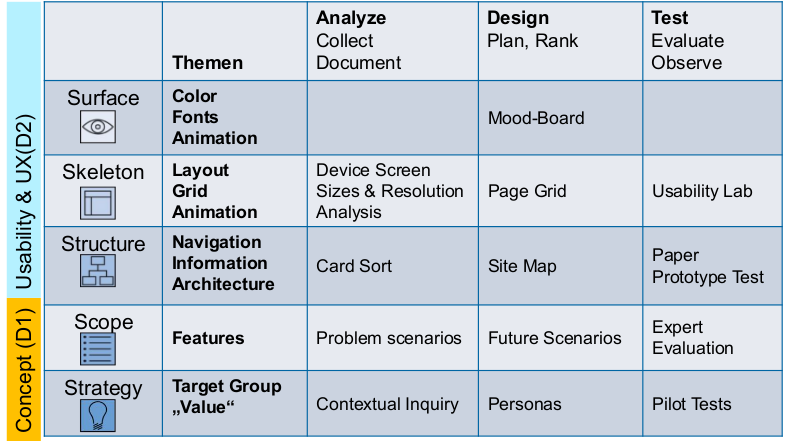
\includegraphics[width=.25\textwidth]{figures/ucdIssuesTechniques.png}
\end{breakbox}

\begin{breakbox}
\boxtitle{Process} 

\begin{itemize}
\item
  Going in direction \textbf{from Down to Up}
\item
  Which strategy do you want to go for? Which personas are your target?
\item
  Which features do you want to support? Explain it with future
  scenarios.
\item
  Once you know the target group and the features, you can think about
  the structure of the app. How do I get to which feature?
\item
  After the structure, we need to think about different screens and
  their layout.
\item
  And finally color, fonts and animations need to be defined.
\end{itemize}

\end{breakbox}

\subsection{Techniques for a good structure}

\begin{breakbox}
\boxtitle{Card Sort} 

Card Sort is a useful technique to determine navigation hierarchies and
naming of menu item.

\textbf{Open Card Sort}: Start with content cards. Let future users
create groups and name them (5+ users).\\
\textbf{Closed Card Sort}: Start with content cards and group labels.
Let future users match content cards to group labels.

\end{breakbox}

\columnbreak
\begin{breakbox}
\boxtitle{Screen Map} 

The ``Screen Map`` for an App lists all screens of an App, groupings and
major navigation links.

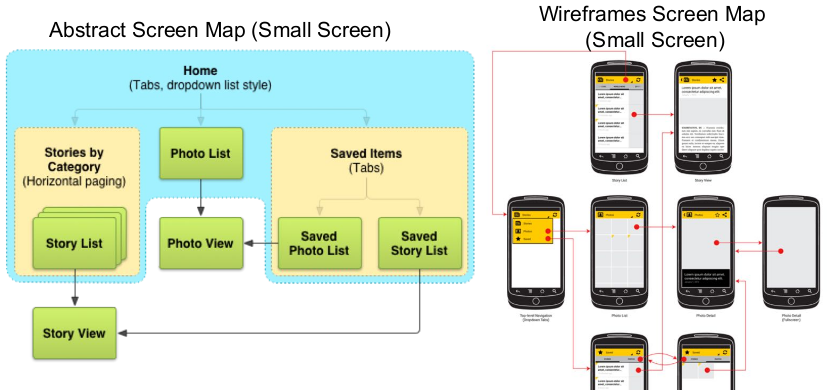
\includegraphics[width=.25\textwidth]{figures/screenMap.png}

A screen Map is not the same as a screen flow. You can see the
Screen Map as a class diagram in UML, while the Screen Flow would be a
object diagram. In the Screen Flow, all instances of each view are
visible.

\end{breakbox}

\begin{breakbox}
\boxtitle{Prototyping / Usability Testing} 

\begin{itemize}
\tightlist
\item
  Defining good Scenarios with plausible needs, goals, context, trigger,
  persona (skill profile)
\item
  Creating inexpensive/quickly the needed screen flows for testing
  (paper or interactive)
\item
  Creating matching task-descriptions that communicate needs, goals,
  context, trigger, but not steps
\item
  Inviting the right test-persons
\item
  Making test persons understand that the system/concept is tested
\item
  Make test persons ''Think Aloud''
\end{itemize}

\end{breakbox}

\begin{breakbox}
\boxtitle{Usability Testing - Test Tasks} 

\begin{itemize}
    \item Scenarios are the basis for creating screen flows and description of the test tasks.
    \item Test tasks specify the users context, need, goal and trigger
    \item Tasks do NOT specify specific steps that should be taken
\end{itemize}

\end{breakbox}

\begin{breakbox}
\boxtitle{Usability Testing - Test Tasks Example} 

\textbf{Invited Test Person:} \\
Should be bread-lovers ... \\
\textbf{Task 1 Description (includes more, but also)} \\
This morning you finished the last piece of bread. You 
made a mental note that you should remember buying 
a fresh loaf of your favorite St 
Galler
bread in the 
evening.
Assume that you have been using the Breadwinner 
App already for a while. The app is tracking you buying 
patterns. 
Assume that it is lunch time and before starting your 
afternoon's work you check your phone. Your home 
screens shows the following message. Proceed to 
preorder (???) your bread for the evening. \\
\textbf{Task 1 Step 2:} \\
Assume that it is 6PM you just exited the train to 
return home 
-
please check your phone. 
[Do you understand why it was sent?]  \\
\textbf{Task 1 Step 3:} \\
You just arrived at the bakery. Please pick up (???) 
your preordered (???) bread. Please also buy and pay 
for the pastry that is offered as "special offer" to regular 
customers.

\end{breakbox}

\begin{breakbox}
\boxtitle{Usability Testing - Mistakes} 

\begin{itemize}
\tightlist
\item
  Recruiting unsuitable participants
\item
  Not testing early and often during the project lifecycle
\item
  Following too rigid a test plan
\item
  Not rehearsing your setup
\item
  Using a one-way mirror
\item
  Not meeting participants in reception
\item
  Asking leading questions
\item
  Undertaking two roles in a testing session
\item
  Not considering external influences
\end{itemize}

\end{breakbox}


\subsection{Surface \& Skeleton}

\begin{breakbox}
\boxtitle{Designing for the human body / Physiology} 

The screen size is getting bigger, but your finger is still the same.
The region you don't reach is getting bigger, so you need to rearrange
the things according to this fact (e.g.~menu at the bottom).

\end{breakbox}

\begin{breakbox}
\boxtitle{Designing for the human mind} 

Place things there where a user expects to see something (e.g.~error
message at a reasonable place).

\end{breakbox}

\begin{breakbox}
\boxtitle{Mobile design patterns} 

\begin{itemize}
\tightlist
\item
  Using empty screens for the introduction into the app
\item
  Coach marks to show the usable gestures or actions
\item
  Try to replace dropdowns by other menus, like a switch or a slider
\item
  Using skeletons to make the app feel faster?
\end{itemize}

\end{breakbox}


\hypertarget{platform-guidelines-for-android}{%
\subsection{Platform Guidelines for
Android}\label{platform-guidelines-for-android}}

\begin{breakbox}
\boxtitle{Material Design} 

Material Design stands for paper form, or how it should look
like.
\end{breakbox}

\columnbreak
\begin{breakbox}
\boxtitle{Elevation hirarchy} 

Elevation hirarchy means, that components are physically stacked. So some elements are over the other elements and create for instance with that shadows.

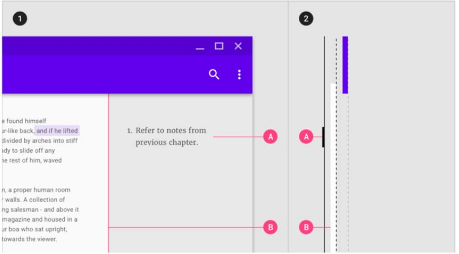
\includegraphics[width=0.2\textwidth]{figures/elevationHirarchy.png}
\end{breakbox}

\begin{breakbox}
\boxtitle{Motions} 

Motions are described as well. How shold the screen move or
behave?\\
\textbf{Bottom navigation} is the new way to go.\\
More things which are described: 
\begin{itemize}
    \item Permissions
    \item Widgets
    \item About sections
\end{itemize}
\end{breakbox}

\begin{breakbox}
\boxtitle{Android Anti-Patterns} 

\begin{itemize}
\tightlist
\item
  The splash screen\\
  better: use image placeholders
\item
  The tutorial screen\\
  better: explain just in time, in context
\item
  The (pre-operation) confirmation window\\
  better: provide undo (notification)
\item
  On-screen Back button\\
  If necessary provide on-screen up button
\item
  Menu button (outdated)
\item
  Hiding the status bar
\item
  Swipe overlay quick actions
\item
  Using non-Android designs
\end{itemize}

\end{breakbox}
